\documentclass[12pt]{article}
% \usepackage[right=1.25in,left=1.25in,top=1.1in,bottom=1.1in]{geometry}
\usepackage{graphicx}
\usepackage{indentfirst}
\usepackage{setspace}
\linespread{1.6}
\usepackage{hyperref}
\hypersetup{
colorlinks=true,
    linkcolor=black,
    filecolor=black,      
    urlcolor=blue,
    citecolor=black,
}
\usepackage[letterpaper, portrait, margin=1in]{geometry}
\usepackage{bbm}
\usepackage{dcolumn}
\usepackage{appendix}
\usepackage{subcaption}

\usepackage[para,online,flushleft]{threeparttable}

\usepackage{natbib}
\def\citeapos#1{\citeauthor{#1}'s (\citeyear{#1})}

\usepackage{amsfonts}
\usepackage{amsmath,amsthm} 
\usepackage{engord}
\usepackage{float}
% \usepackage{subfig}
\usepackage{pdflscape}
\usepackage{booktabs}
\usepackage{pgfplots}
\pgfplotsset{compat=1.14}
\pgfplotsset{every axis label/.append style={font=\tiny}}
% \usepackage[labelsep=period]{caption} %% This switches "Table 1: Title" to "Table 1. Title"

\usepackage{amssymb} %% Necessary, just for the \checkmark command  in tables.
\usepackage{multirow} %% Necessary if we are doing tables in LaTeX

\usepackage{xr}

\usepackage{setspace}
\onehalfspacing

\usepackage{sectsty}
\sectionfont{\large}
\subsectionfont{\normalsize}
\subsubsectionfont{\normalsize}

\newcommand{\specialcell}[2][c]{\begin{tabular}[#1]{@{}l@{}}#2\end{tabular}}

\usepackage{appendix}
% % for the figure
% \usepackage[english]{babel}
% \usepackage{graphicx}
% \usepackage[letterpaper]{geometry}
% \geometry{top=1.0in, bottom=1.0in, left=1.5in, right=1.0in}
% \usepackage{flafter} % make sure figures do not appear before their text
% \usepackage{sidecap} % use side captions for floats
% \usepackage{subfig} % subfloats
% \usepackage{float}
% \usepackage[caption = false]{subfig}
% \usepackage[demo]{graphicx}
%%%%%%%%%%%%%%%%Title%%%%%%%%%%%%%%%%%%%%%%%%%%%%%%%%%%%%%

\title{ \vspace*{-2.5cm} \hspace*{Social Norms in Public Provision vs Appropriation Game}}

% Information for title page
\author{Jancy Ling Liu\thanks{School of Economics, Georgia Institute of Technology, 221 Bobby Dodd Way, Atlanta, Georgia 30332, \href{mailto:jancyll@gatech.edu}{jancyll@gatech.edu}.} }
\date{\today}

\begin{document}

\maketitle

\begin{abstract}
\singlespacing \noindent The current literature have shown the effects of social norms on promoting varied pro-social behaviors. The multiple types of norms information may work differently, however, by the way they are presented to consumers. This paper investigate the effect of social norms, which includes injunctive norms, descriptive norms, and working-together normative appeals, on the consumption behaviors of eco-labeled products. I conduct a choice survey to investigate how different types of social norms work associated with multiple eco-labels. I use different level of descriptive norms information and eco-labels as attributes in a series of choice set. I randomly assign injunctive norms message and working-together normative appeals message as treatments. The results show the price premium exist for eco-labels and descriptive norms start to work at the 50-percent level. The willingness to pay increases from one label to three labels when presented to consumers. Further, under injunctive norms and working-together normative appeals treatments, the willingness to pay for both descriptive norms information and certified eco-labels increase. These results demonstrate how to use norms information to improve eco-labels’ performance to promote green consumption and environmental improvement.

\end{abstract}

\newpage
% make the section on the left 
\section{Introduction 
\label{sec:introduction}}

Social norms have gained more extensive attention in recent literature. Empirical results show that social norms can create non-monetary incentives to spur pro-social behaviors, even when paying a price premium \citep{carlsson2010conformity, allcott2011social, torres2018direct}. Lab experiments show that social norms can affect conditional cooperation in the one-shot public good game \citep{fehr2018normative,fischbacher2001people}. These lead to a question about the potential of social norms to overcome free-rider problems facing social dilemmas. 

Social dilemmas indicate a situation when individuals face a choice of strategies to either contribute to their self-interest or group interests. In empirical studies about social norms, we can see this type of social dilemmas exiting in some contexts. For example, in \cite{allcott2014short} ’s home energy project, consumers significantly decrease their energy consumption after the treatment of injunctive norms. In another word, after the treatment of norms information, consumers trade off their self-interests of energy use in exchange of the group benefits of reducing energy consumption. This role of social norms has been studies in water consumption \citep{ferraro2011persistence,ferraro2013using, torres2018direct}, recycling\citep{schultz1999changing}, hotel towel use\citep{goldstein2008room}, charity giving \citep{croson2008impact,krupka2016differential}, and sustainable transportation \citep{kormos2015influence}. 

Public provision game is a general format for this type of problem facing social dilemmas. Agents have to decide how much they want to contribute to the group funds while sacrificing their benefits. Most literature found that in a finite period, participants decrease their contributions along with the time \citep{fischbacher2010social,kandul2021public}. Its paired game is the appropriation game, where participants need to decide how much they extract from the group fund. Both games create a common pool based on the group fund that each group member equally shares. The different rewards between the contribution in the group fund and individual fund lead to a social dilemma for agents to trade off their interests with the group interests. 

These social dilemmas gain increasing interest in environmental economics since it reflects the natural conflicts in real life. \cite{fischbacher2001people} has shown that information of in-group member contribution will lead to corresponding conditional cooperation in the public provision game, leading to an increasing contribution to the public fund. \cite{fehr2018normative} summarizes these findings and emphasizes the importance of cooperation and how it can solve the social dilemmas problem. In 2021,  \cite{kandul2021public} tries to use out-group descriptive norms feedback to explore its effect on the contribution given by the agents. They directly give subjects feedback about if their contribution is above, below, or equal to their out-group members' contribution. This feedback leads the subjects to adjust their contribution to the average line and does not show any effects to solve the social dilemmas' problems.  In their results, the average contribution under feedback information treatment is lower than the control group. 

It is currently controversial about the effects of social norms in the public provision game. There are concerns in empirical studies about the effects of social norms as well. \cite{pellerano2017extrinsic} reports social norms backfire when adding price salience on electricity consumption. All these lead to the question about the effects of social norms in social dilemmas setting. When we apply social norms as non-monetary incentives, it is essential to understand their effects in a broader framework and test its generosity. Public provision and appropriation games offer an excellent framework to study social norms in a general sense.

This paper aims to test the effects of social norms in public provision and appropriation games. Specifically, it tries to test three types of social norms and their effects. Economists are more familiar with descriptive norms and injunctive norms. Descriptive norms indicate the perceptions of what is commonly done in a given situation. Injunctive norms indicate the perceptions of what is commonly approved or disapproved within the culture \citep{reno1993transsituational}. \cite{sparkman2017dynamic} points out the effects of dynamic norms, showing the perception of trending behaviors within a group, on meat consumption even under the contrary static norm. \cite{sparkman2021social}  argues that dynamic norms can be used to drive collective action in the fight against climate change, even under a negative current norm. However, there is not much evidence of dynamic norms existing in recent literature, and it is not sure how their effects apply in broader contexts.

This paper tests the effects of descriptive, injunctive, and dynamic norms in public provision and appropriation games. Employing the repeated linear provision game, we assign subjects into ten groups with each group of four subjects. Subjects are informed to choose an amount to contribute to the group fund simultaneously. After the baseline game, we will apply the "strategy method" to elicit subjects' contribution preferences \citep{fischbacher2001people}. In the following sessions, subjects in the control group will only have the information about their payoff after every session, which indicates the average in-group contribution.
Meanwhile, subjects in the treatment group will receive out-group contribution as norms information before their contribution decision. The out-group norms information include three treatment. The first treatment is the out-group descriptive norms treatment. Under this treatment, the subject will receive the out-group median contribution information solely before their decisions. The following treatment is out-group injunctive norms treatment, with which the subjects will receive individual feedback compared to the out-group information with the valence of emotion. Following \cite{kandul2021public}, this information will indicate if subjects' contribution is "below", "above", or "equal to" the out-group average. The valence of emotion aims to show if their contributions are approved or disapproved in the big group \citep{schultz2007constructive, allcott2011social}. The last treatment is the out-group dynamic norms treatment. The subjects will receive trending norms information before their contribution. This trending norms information will only elicit positive information about the percentage of participants increasing their contribution in the past sessions. The out-group dynamic norms treatment will be repeated five sessions, while subjects do not know when they will end this game. 

Under this setting, we can test the effects of different types of social norms in volunteer contribution and check the heterogeneity of the norms effect based on their initial contribution preference elicited from the "strategy method". \cite{cox2013provision} shows provision and appropriation games are payoff-equivalent and appropriation games shows lower efficiency under power asymmetry setting. Since the key treatment offered in this study is the out-group information. In a paired appropriation game, the norms information might encourage subjects' choice of free riding and lead to more over-exploitation. 

This paper contributes to the literature in three ways. First, it aims to solve the free riders problem that commonly exists in common-pool in provision game and identify the over-exploitation problem under appropriation game. By varying the different social norms information, it tries to check the heterogeneity of social norms effects under the provision and appropriation games. Second, it aims to support the emerging empirical evidence of social norms and explore its generosity in classical games. Third, it evaluates the effects of norms on different types of subjects with preference heterogeneity. 


\section{Social norms and Conditional cooperation in Provision game}

As a contribution game, the public provision game offers a space where $N$ agents decide the amounts they plan to contribute to a group fund from their endowed private fund. The group fund will distribute equally to all agents in the end, no matter how much they contribute. The final payoff of each agent is a combination of their left private fund and the equal share they get from the group fund. Each agent $x_i$ begins with e “tokens” in their private fund and chooses an amount $c_i$ from the finite set $ \{ 0, 1, 2, … e \}$ to contribute to the group fund. Each token or experimental money indicates a certain amount of real payoff \$G. Each token contributed to the group fund decreases the value of the individual fund of $x_i$ by \$1 and increases the group fund by \$M, where $N>M>1$. Then the money payoff to an agent $i$ is:

\begin{center}
$
\pi_p^i = e - c_i + M \sum^N_{j=1} \frac{c_j}{N}
$
\end{center}

There exists a social dilemma since $N>M>1$. Under homo economicus preferences, the dominant strategy for agents is to contribute zero to the group fund. Then the average payoffs of agents will be \$e. \cite{cox2013provision} show that the average group earnings are higher than the homo economicus preferences for one-time simultaneous provision game. In the repeated public provision games, the previous literature show that the average contribution decreases \citep{fischbacher2010social, kandul2021public}.

\cite{fischbacher2001people} explores conditional cooperation using strategy methods in public provision games. The information it offers to participants solely includes all the possible average contributions of other group members. \cite{fischbacher2010social} replicated these results. Using strategy method, they find that with the increasing contribution of other group members, there are 55 percent "conditional cooperators" who linearly increase their contributions, 23 percent "free riders" who are irrespective of other members' contribution, 12 percent "triangle contributors" who increase their contributions to a point and then decreases their contributions, and 10 percent unclassified subjects.

\cite{fehr2018normative} explores the possibility of social norms shaping human cooperation. However, in \cite{kandul2021public}'s work to analyze the effects of payoff-irrelevant out-group feedback as descriptive norms on provision game, they find that the treatments group has an overall lower average contribution compared to the baseline group. It shows that norms information makes subjects adjust their behaviors based on out-group average contribution and decrease the overall efficiency of the game. 

Social norms have at least three categories in current literature shown in economics. Descriptive norms show the prevalence of other people’s behaviors within a group. The second norm is injunctive norms that show approval or disapproval of specific behavior within a social context. The recent one is called dynamic norms, which show the perception of certain behaviors within a group. The previous two have been shown can create social learning and lead to conditional cooperation \citep{cai2009observational,alpizar2008anonymity}. The last one has also been shown to increase people’s adoption of the new trending behaviors after showing them the dynamic norms information \citep{sparkman2017dynamic}. \cite{sparkman2021social} argues that dynamic norms primarily work for collective action like fighting for climate change.

These observations leads to the following hypothesis related to the effects of social norms under public provision game (PG):

Hypothesis 1: 
The out-group descriptive norms information increases the contribution to the Group Fund in PG.

Hypothesis 2:
The out-group injunctive norms information decreases the contribution to the Group Fund in PG. 

Hypothesis 3:
The out-group dynamic norms information increases the contribution to the Group Fund in PG.

\section{Asymmetric incentives in provision and appropriation game}

Appropriation game (AG) creates a please where $N$ agents choose how much they extract from a group fund. Under this setting, the agents start with an endowed group fund $E = Ne$ tokens. This group fund has value \$ME. Each agent extract an amount $a_i$ from the set $\{0,1,2,…,e\}$ from the group fund. Each token worth \$M in group fund while worth \$1 in individual fund, where $N>M>1$. Each agents’ payoff equal to a combination of their individual fund and the equally share from the remaining value of the group fund. The money payoff to an agent $i$ under appropriation game is:

\begin{center}
$
\pi_i^a=a_i+M(E-\sum_{j=1}^N a_j )/N
$
\end{center}

\cite{cox2013provision} shows that for the one-shot game, the average earnings across PG and AG are very similar. It holds in a sequential boss game. Only when agents have asymmetric power in the sequential game, the group earnings will significantly lower than the same setting in PG. 
When we conduct a paired treatment under AG, the treatment information might offer asymmetric incentives for subjects to contribute. Specifically, the same types of norms treatment shown in PG might spur more extraction from the group fund as "bad social norms" under AP. So I hypothesize reverse effects of social norms under AG: 

Hypothesis 4: 
The out-group descriptive norms information increases the extraction to the Group Fund in Provision Game.

Hypothesis 5:
The out-group injunctive norms information decreases the extraction to the Group Fund in Provision Game. 

Hypothesis 6:
The out-group dynamic norms information increases the extraction to the Group Fund in Provision Game.


\section{Experiment design }

To study the research question and test these hypotheses, I plan to conduct five stages paired game of PG and AG. Participants will be recruited from undergraduates with a wide range of disciplines. Forty subjects will be in one session simultaneously, and they will be privately and anonymously assigned to 10 four-person groups via the computer. Subjects cannot identify their group members in the room. Participants will be noticed that their group members will change in every stage to avoid reputation problems. 

Subjects will start with a one-shot provision game as Stage 1, where four agents contribute to the group fund simultaneously. Then the participants will play the same game under the strategy method (Stage two), where each player contributes the token to the group fund based on all possible average contributions from other group members. 

After these two baseline games, subjects will be randomly assigned to the treatment and control groups (20 \% of subjects will be in the control group). Subjects in the control group will solely receive information about their payoff from their previous session, while each subject in the treatment group will face treatments before their moves. In stage three, agents in the treatment group will be revealed the out-group descriptive norms feedback from Stage 1. Here out-group descriptive norms mean “60 \% of participants contribute $x$ averagely to the group fund”. Then in stage four, they will be shown the out-group injunctive norms feedback, which is the individual feedback to show if their previous contribution is above, below, or equal to the average contribution of the out-group members from Stage three. The valence of the emotion will be used as injunctive norms. 

In stage five, the subjects will be revealed the trending information of cooperators from previous stages (except stage two) as out-group dynamic norms treatment. The trending information indicates the percentage of participants who have ever increased their payoff once in the past three sessions. Stage five will play five times, while subjects do not know when the game will end. 

In the beginning of each session, subjects will privately read a set of instructions that clarifies their roles and treatment (See Appendix A). They will receive double-blind payoff protocol based on their accumulated payoff in all runs. 

\section{Pilot Results}

From the pilot experiment, I collect the data from eight participants. The first session concerns subjects' contribution decisions corresponding to the "contribution table", which shows their elicited willingness to contribute given the average contribution level of other members. Figure \ref{fig:con_con} shows results of subjects' conditional contributions. Consistent to \cite{fischbacher2001people}'s study, the results indicate most subjects show conditional cooperation since their contribution is increasing and matching with the contributions of others. There is also few subjects who are free riding since they submit a contribution that contains 0 in all 21 entries. 

\begin{figure}[ht]
    \centering
    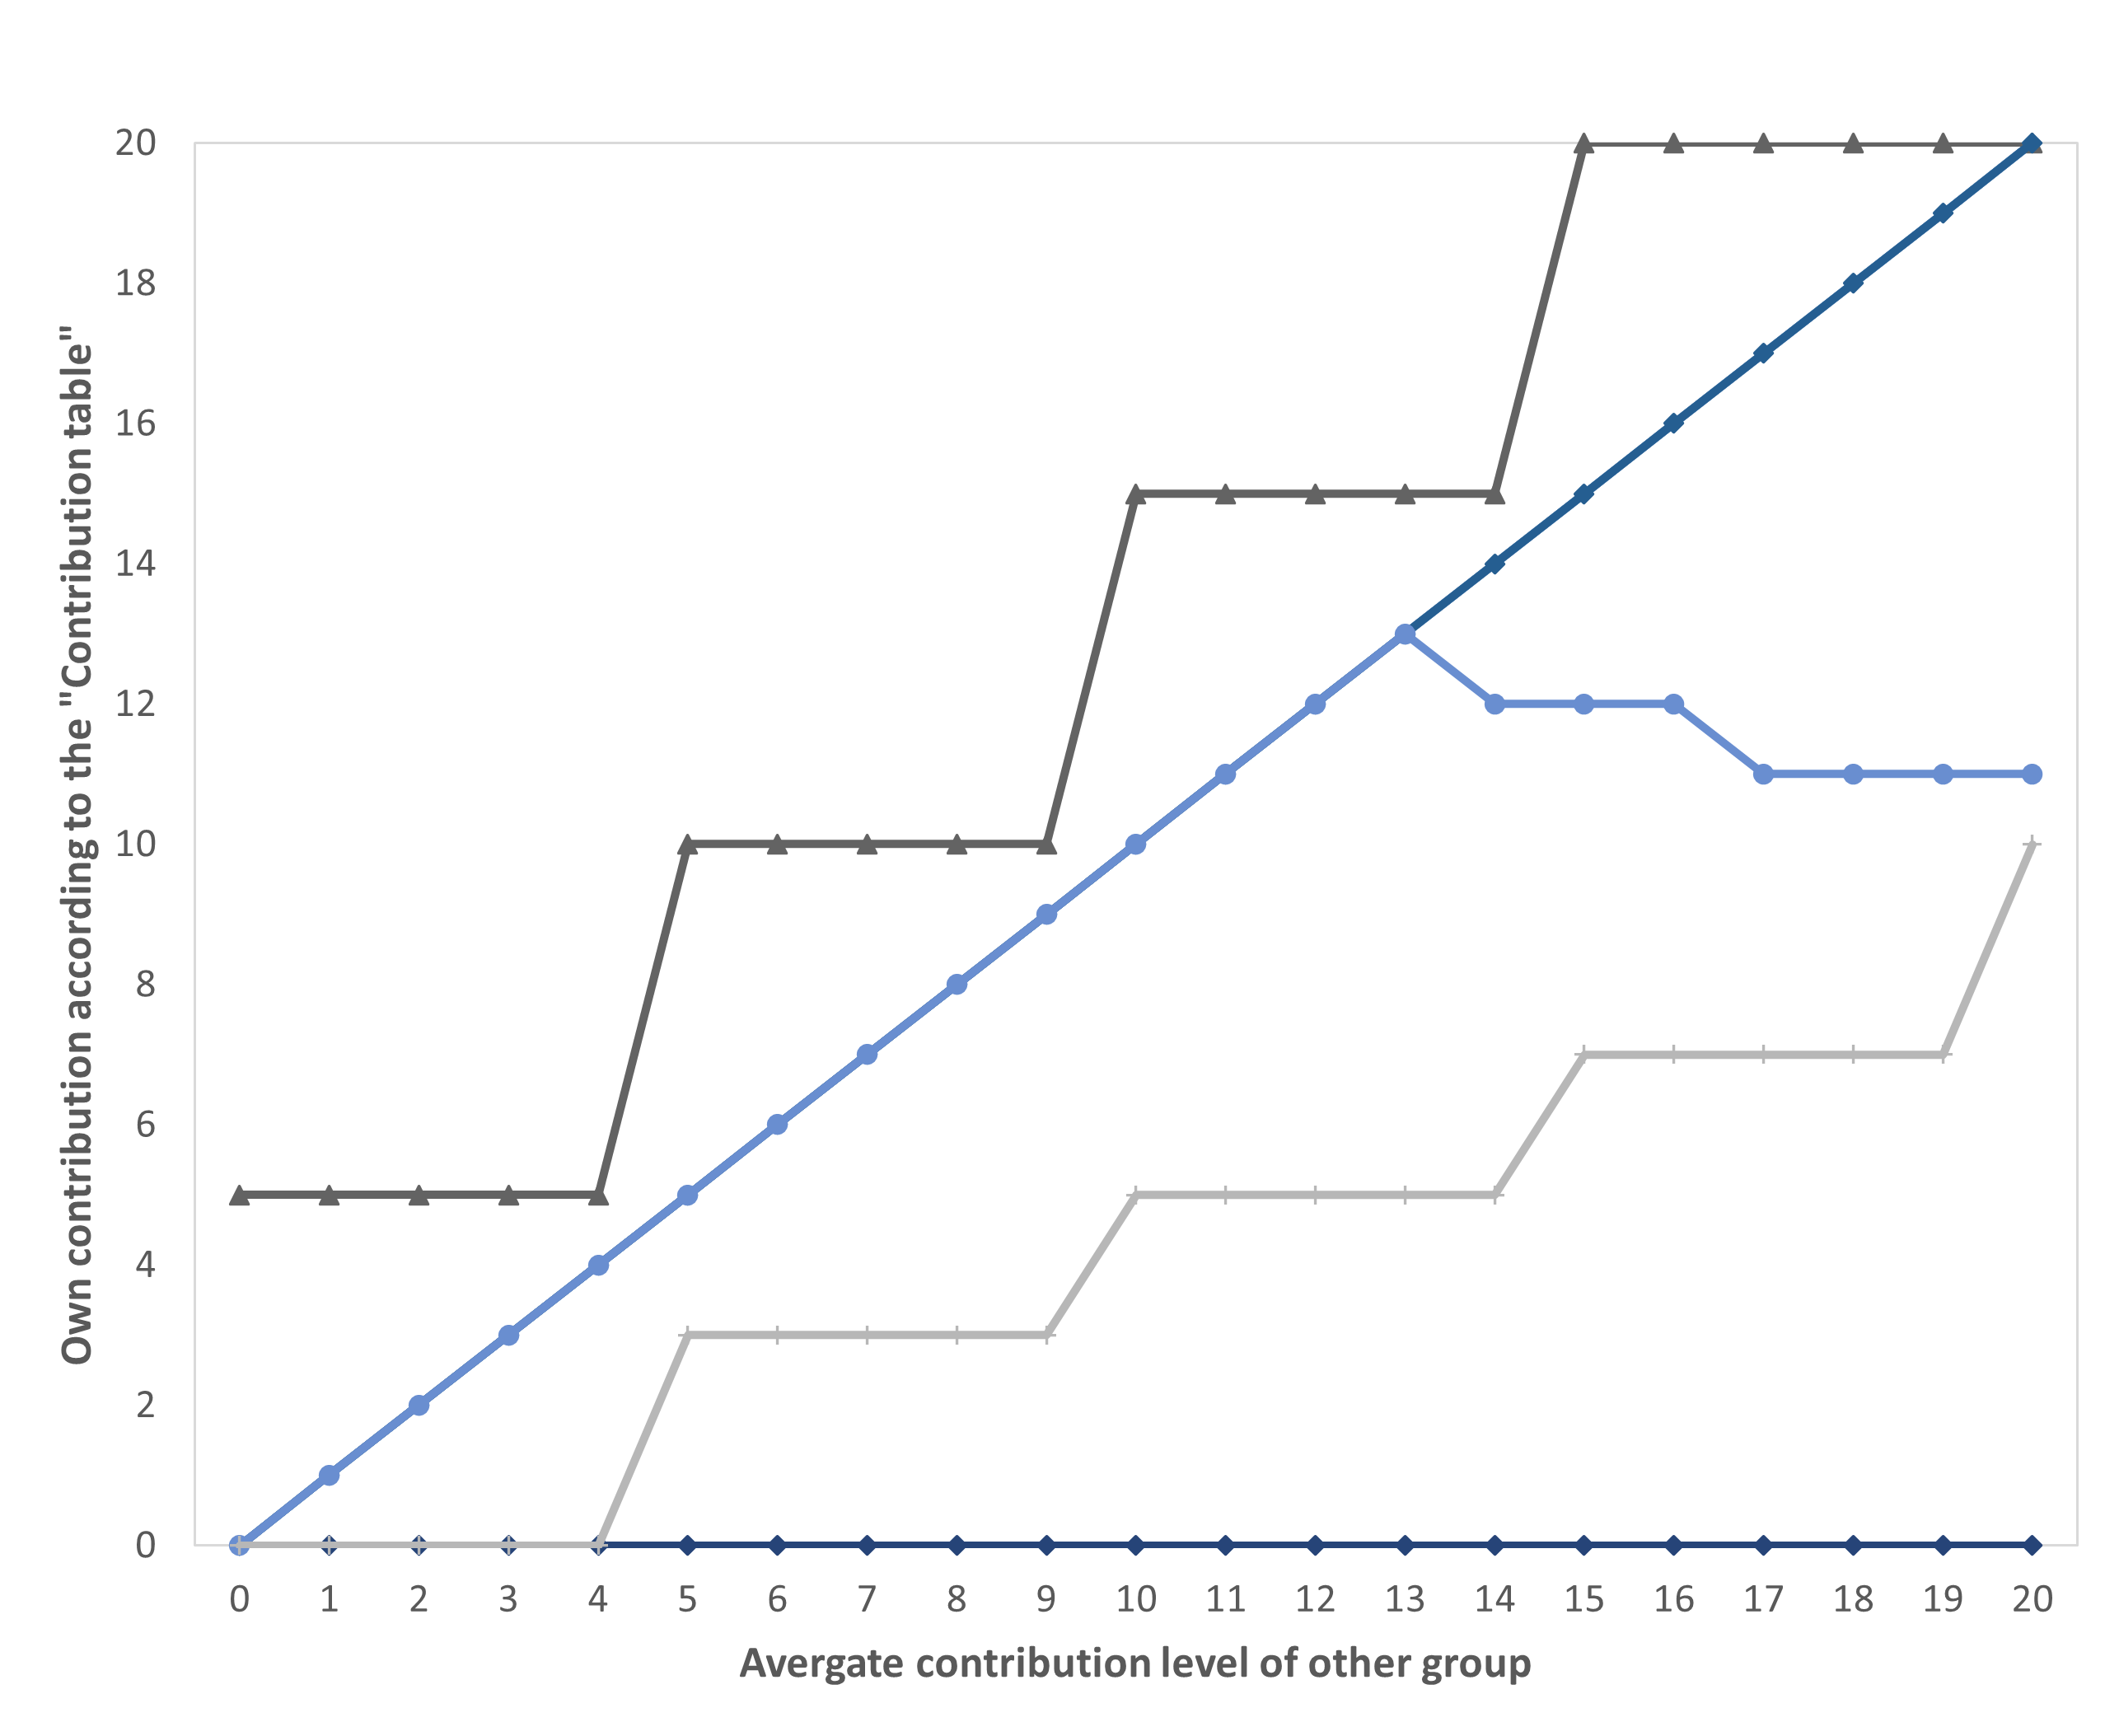
\includegraphics[scale = 0.7]{con_con.png}
    \caption{Own Contribution level for each average contribution level of other members}\label{fig:con_con}
\end{figure}



\begin{figure}[ht]
    \centering
    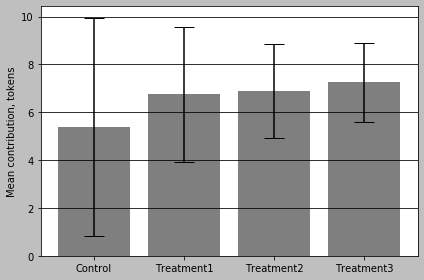
\includegraphics[scale = 0.9]{bar_plot_with_error_bars_!.png}
    \caption{Average contributions under different treatments}\label{fig:avg_con}
\end{figure}

\begin{figure}[ht]
    \centering
    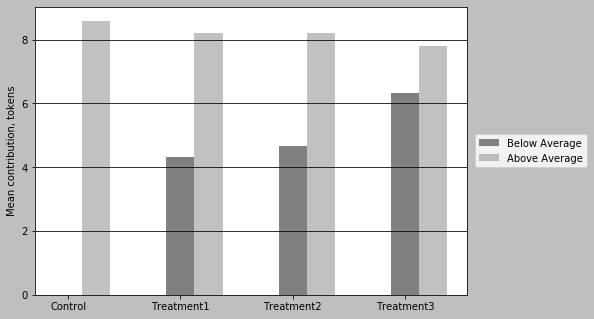
\includegraphics[scale = 0.9]{compare.png}
    \caption{Average contributions under different treatments}\label{fig:compare}
\end{figure}

\section{Conclusions}

This study demonstrates how social norms information can change the contribution in PG and AG and explore its potential to reduce free-riders problems under social dilemmas. Through three types of social norms treatment, it shows the different effects of descriptive, injunctive, and dynamic norms information. It also checks the heterogeneity of these effects based on the different types of contribution preferences. 

The current design has not involved asymmetric power like Boss and King's role in PG and AG as \cite{cox2013provision}. Instead, it follows the baseline design and aims to find the preliminary effects of social norms in PG and AG. However, once we can see the effects of social norms on baseline games, there is more possibility to extend to other versions of PG and AG in the future. 

\newpage

Appendix A. Experimental Instructions

These instructions were printed and delivered to subjects at the same time after all participants arrive. The second movers will receive the social norms treatment information before they decide contribution.
 
Instructions

Welcome and thank you for participating in this experiment. Please turn off your phones and do not talk to other participants. If you have a question, please raise your hand, and the experimenter will come and answer you privately. 

In this experiment, you can earn money except for the participation fees. Your final earnings will depend on your own decisions and the decisions of other participants. 

During the experiment, your earnings will express in Tokens that will be converted at the end of the experiment in Dollars: 1 Token = \$0.15.

You will be randomly and privately assigned to a group of four. There will be more than five rounds in total. After each round, you will be randomly assigned again to a new group with new members. Every member has their private account A in each group, and the group has a group account B. In every group, there are four private accounts A and a single group account B. 

At the beginning of each round, you will receive 40 Tokens. You need to decide how you would like to allocate the 40 tokens between accounts A and B.  For each token you put on your private account A, you will receive exactly one token. For each token you put on the group account B, it will multiply by three. The resulting amount of tokens on account B will be divided equally among four group members. You will receive the payoff from both private account A and your share of the group account B:

Tokens on account A + 0.75* sum of contributions to group account B

Your earnings from account A are independent of the decisions of other group members. Your earnings from group account B depend on the decisions of all group members. No matter how many tokens you contribute to group account B, you will always receive your share equally. After all group members finish their decisions, you will see your payment in that round on the computer screen. 

The information you receive might be varied in each round. After you finish all rounds, the computer will sum up your payment for each round. So, every round of your decision matters for your total payoff.


\clearpage
\printbibliography
\bibliography{works-cited}
\bibliographystyle{chicago}

\end{document}
